% use http://www.tablesgenerator.com/latex_tables
\begin{table}[H]
	\centering
	\begin{tabular}{@{}llr@{}}
		\toprule
		\toprule
		\multicolumn{2}{c}{Item} &            \\ \cmidrule(r){1-2}
		Animal     & Description & Price (\$) \\ \midrule \midrule
		Gnat       & per gram    & 13.65      \\
		& each        & 0.01       \\
		Gnu        & stuffed     & 92.50      \\
		Emu        & stuffed     & 33.33      \\
		Armadillo  & frozen      & 8.99       \\ \bottomrule
	\end{tabular}
	\caption{My caption}
	\label{my-label}
\end{table}

\begin{figure}[H] % Example image
	\center{
\includegraphics[width=0.5\linewidth]{placeholder}}
	\caption{Example image.}
	\label{fig:speciation}
\end{figure}

\lipsum[6] % Dummy text
\begin{wrapfigure}{l}{0.4\textwidth} % Inline image example
	\begin{center}
		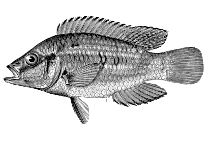
\includegraphics[width=0.38\textwidth]{fish}
	\end{center}
	\caption{Fish}
\end{wrapfigure}
\lipsum[7-8] % Dummy text

\begin{figure}[H]
	\centering
	\subfigure[Original]{
		\begin{minipage}[t]{0.25\linewidth}
			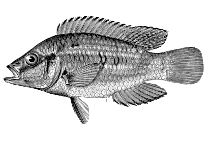
\includegraphics[width=1.4in]{fish}
		\end{minipage}
	}
	\subfigure[SIFT Features]{
		\begin{minipage}[t]{0.25\linewidth}
			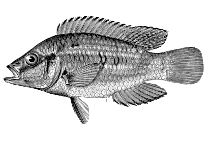
\includegraphics[width=1.4in]{fish}
		\end{minipage}
	}
	\caption{Source Image}
\end{figure}

\begin{description} % Numbered list example
	
	\item[First] \hfill \\
	\lipsum[9] % Dummy text
	
	\item[Second] \hfill \\
	\lipsum[10] % Dummy text
	
	\item[Third] \hfill \\
	\lipsum[11] % Dummy text
	
\end{description} 


%ALGORITHMS
\IncMargin{1em}
\LinesNumbered
\begin{algorithm}[H]
	\SetKwData{Left}{left}\SetKwData{This}{this}\SetKwData{Up}{up}
	\SetKwFunction{Union}{Union}\SetKwFunction{FindCompress}{FindCompress}
	\SetKwInOut{Input}{input}\SetKwInOut{Output}{output}
	
	\KwData{this text}
	\KwResult{how to write algorithm with \LaTeX2e }
	
	
	\BlankLine
	\While{not at end of this document}{
		read current\;
		\eIf{understand}{
			go to next section\;
			current section becomes this one\;
		}{
			go back to the beginning of current section\;
		}
	}
	\caption{How to write algorithms}
	
\end{algorithm}
\DecMargin{1em}
	